% Chapter 5

\chapter{Results} % Main chapter title

\label{Chapter5} % For referencing the chapter elsewhere, use~\ref{Chapter5} 

In this research, we used the offline measurement generator in getting the
measurement across different real-world programs. We calculate the ScaRR control
flow information for each of the programs. We analyze and present the result in
this chapter. The analysis and source code of the program is available in this
Github repository: \url{https://github.com/lamida/scarr-sample-program/}.

We choose four large open-source projects for analysis. We download the latest
version of the source code. The first software is Redis $6.2.4$
~\cite{RedisRedis2021}, a so-called data structure server that is widely used in
the real world. The Redis source build consists of the server binary and the
client command-line interface (CLI). We analyze both of the programs.

The second program we analyze is bzip2 $1.08$~\cite{Bzip2Bzip2}. Bzip2 is a free
and open-source file compression program. The third program is OpenSSL
$1.1.1j$~\cite{OpensslOpenssl2021}. OpenSSL is a full-featured toolkit for TLS
protocol. 

The last suite program we analyze is Coreutils
$8.32$~\cite{CoreutilsCoreutils2021}. Coreutils is a suite of Unix utilities for
file, shell, and text manipulation.

For each of program, we are collecting the following measurements:

\begin{itemize}
    \item source code lines
    \item IR lines
    \item number of basic blocks (nBB)
    \item number of ScaRR measurements (nM)
    \item number of checkpoints (nCP)
    \item number of LoA (nLoA)
\end{itemize}

However, before we go to the result, the following section shows how to run the
pass.

\section{Running The Pass}

To mark the list of Checkpoints, we can invoke LLVM \texttt{opt} as shown in
listing~\ref{listing:mark-cp-in-cfg}.

\begin{listing}[ht]
    \begin{minted}[
        frame=lines,
        framesep=2mm,
        baselinestretch=1.2,
        fontsize=\footnotesize,
    ]{bash}
        opt -passes=scarr-cp-marker <file>.ll
    \end{minted}
    \caption{Mark Checkpoint in BasicBlock.}    
    \label{listing:mark-cp-in-cfg}
\end{listing}

We can see the output of the basic block that has been marked with checkpoint using
LLVM \texttt{dot-cfg} pass.

\begin{listing}[ht]
    \begin{minted}[
        frame=lines,
        framesep=2mm,
        baselinestretch=1.2,
        fontsize=\footnotesize,
    ]{bash}
        opt -passes=scarr-cp-marker,dot-cfg <file>.ll
    \end{minted}
    \caption{Print Checkpoints in CFG dot file.}    
    \label{listing:cp-to-cfg}
\end{listing}

The commands in listing~\ref{listing:cp-to-cfg} generates different dot files
per function. We can use \texttt{xdot} command line from Graphiz to see the
graph. 

To mark the list of actions between checkpoints, we can invoke LLVM \texttt{opt}
as shown in Listing~\ref{listing:get-loa}

\begin{listing}[ht]
    \begin{minted}[
        frame=lines,
        framesep=2mm,
        baselinestretch=1.2,
        fontsize=\footnotesize,
    ]{c++}
        opt -passes=scarr-cp-marker,scarr-loa-collector <file>.ll
    \end{minted}
    \caption{Get List of Actions}    
    \label{listing:get-loa}
\end{listing}

Note that we have to run \texttt{scarr-cp-marker} before
\texttt{scarr-loa-collector}.

We discuss the result and its interpretation in the next chapter.


\section{ScaRR Control-Flow Result}

\begin{figure}[htbp]
    \centerline{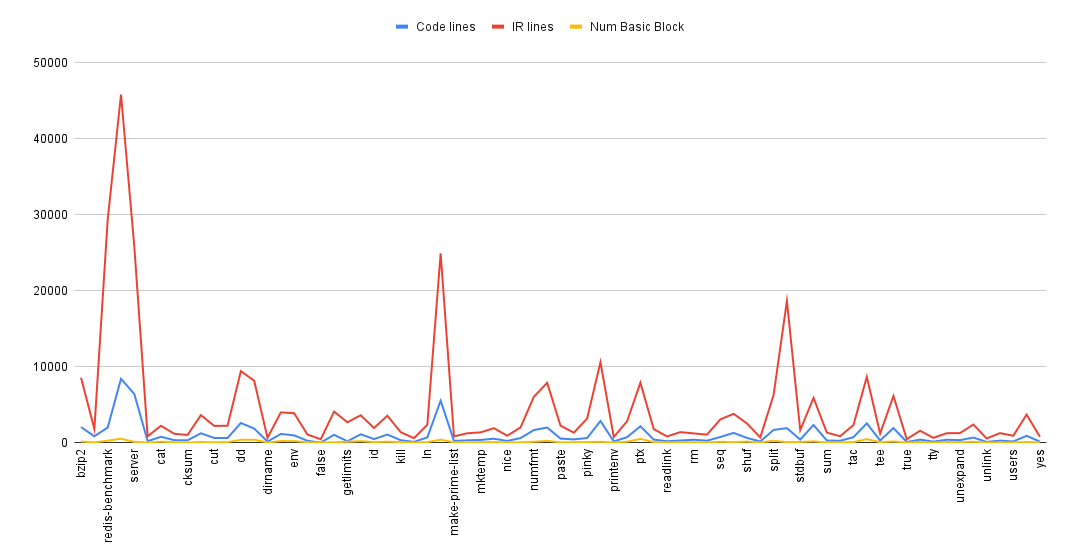
\includegraphics[scale=.55]{Figures/05/code-lines-chart.png}}
    \caption{Lines of Code, Lines of IR and Number of BasicBlocks.} 
    \label{fig:code-lines-chart}
\end{figure}

\begin{figure}[htbp]
    \centerline{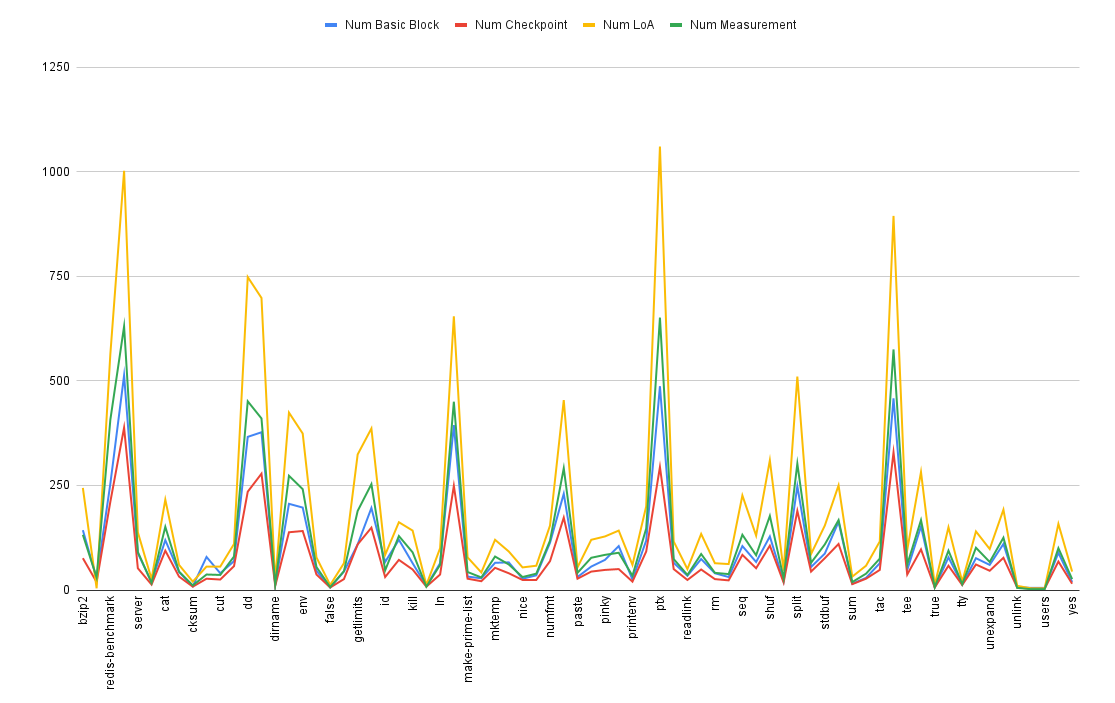
\includegraphics[scale=.55]{Figures/05/bb-chart.png}}
    \caption{Basic Block and ScaRR Control-Flow Result.} 
    \label{fig:bb-chart}
\end{figure}

\begin{table}
    \centering
    \rowcolors{1}{}{lightgray}
    \begin{tabular}{lrrrrrr}
    \toprule 
    Program         & CL         & IRL & BB & M & CP & LoA  \\
    \midrule
    basename        & 190        & 827      & 19              & 17              & 13             & 26       \\
    cat             & 767        & 2215     & 119             & 151             & 94             & 216      \\
    chgrp           & 319        & 1158     & 43              & 44              & 32             & 60       \\
    cksum           & 310        & 1012     & 9               & 11              & 8              & 20       \\
    cp              & 1226       & 3619     & 79              & 37              & 27             & 56       \\
    cut             & 609        & 2196     & 40              & 36              & 25             & 56       \\
    date            & 604        & 2223     & 69              & 80              & 57             & 110      \\
    dd              & 2581       & 9420     & 366             & 451             & 235            & 748      \\
    df              & 1847       & 8146     & 377             & 410             & 278            & 698      \\
    dirname         & 136        & 635      & 13              & 13              & 10             & 20       \\
    du              & 1140       & 3973     & 206             & 273             & 138            & 424      \\
    env             & 952        & 3875     & 197             & 241             & 141            & 374      \\
    expand          & 238        & 1057     & 46              & 55              & 37             & 78       \\
    false           & 2          & 442      & 6               & 7               & 6              & 12       \\
    fmt             & 1029       & 4083     & 44              & 45              & 26             & 64       \\
    getlimits       & 172        & 2681     & 109             & 189             & 109            & 324      \\
    head            & 1095       & 3596     & 196             & 253             & 149            & 386      \\
    id              & 464        & 1922     & 67              & 47              & 31             & 84       \\
    install         & 1059       & 3545     & 120             & 129             & 72             & 162      \\
    kill            & 314        & 1376     & 64              & 90              & 49             & 142      \\
    link            & 93         & 581      & 10              & 8               & 8              & 12       \\
    ln              & 681        & 2350     & 64              & 60              & 37             & 100      \\
    ls              & 5520       & 24925    & 394             & 450             & 249            & 654      \\
    make-prime-list & 230        & 813      & 32              & 43              & 27             & 78       \\
    mkdir           & 296        & 1230     & 28              & 30              & 21             & 42       \\
    mktemp          & 350        & 1347     & 65              & 80              & 53             & 120      \\
    mv              & 512        & 1903     & 66              & 61              & 40             & 92       \\
    nice            & 221        & 905      & 27              & 31              & 24             & 54       \\
    nl              & 596        & 1994     & 35              & 39              & 24             & 58       \\
    numfmt          & 1651       & 6036     & 113             & 118             & 69             & 154      \\
    od              & 1987       & 7876     & 230             & 291             & 173            & 454      \\
    paste           & 530        & 2234     & 31              & 41              & 27             & 54       \\
    pathchk         & 422        & 1306     & 56              & 77              & 44             & 120      \\
    pinky           & 602        & 3161     & 72              & 84              & 48             & 128      \\
    pr              & 2848       & 10596    & 105             & 89              & 50             & 142      \\
    printenv        & 154        & 742      & 25              & 34              & 20             & 60       \\
    printf          & 715        & 2811     & 118             & 147             & 92             & 200      \\
    ptx             & 2153       & 7888     & 487             & 651             & 294            & 1060     \\
    pwd             & 394        & 1777     & 65              & 74              & 50             & 116      \\
    readlink        & 178        & 813      & 34              & 36              & 24             & 50       \\
    realpath        & 278        & 1382     & 74              & 86              & 49             & 134      \\
    rm              & 373        & 1213     & 40              & 41              & 26             & 64       \\
    rmdir           & 253        & 1048     & 31              & 38              & 23             & 62       \\
    seq             & 736        & 3057     & 105             & 132             & 84             & 226      \\
    shred           & 1279       & 3789     & 67              & 83              & 52             & 130      \\
    shuf            & 615        & 2524     & 128             & 177             & 106            & 310      \\
    sleep           & 146        & 688      & 21              & 28              & 18             & 46       \\
    split           & 1668       & 6262     & 248             & 302             & 189            & 510      \\
    stat            & 1907       & 18653    & 55              & 65              & 44             & 86       \\
    stdbuf          & 394        & 1644     & 87              & 109             & 76             & 154      \\
    stty            & 2322       & 5885     & 163             & 167             & 110            & 250      \\
    sum             & 273        & 1312     & 15              & 19              & 14             & 32       \\
    sync            & 239        & 838      & 29              & 39              & 27             & 58       \\
    tac             & 713        & 2324     & 64              & 75              & 48             & 116      \\
    tail            & 2537       & 8657     & 458             & 575             & 329            & 894      \\
    tee             & 278        & 1193     & 48              & 61              & 37             & 96       \\
    tr              & 1914       & 6139     & 152             & 167             & 97             & 282      \\
    true            & 80         & 441      & 6               & 7               & 6              & 12       \\
    truncate        & 388        & 1564     & 78              & 94              & 58             & 150      \\
    tty             & 133        & 624      & 13              & 14              & 12             & 20       \\
    uname           & 376        & 1236     & 76              & 101             & 61             & 140      \\
    unexpand        & 326        & 1255     & 60              & 67              & 46             & 98       \\
    uniq            & 662        & 2379     & 110             & 125             & 77             & 192      \\
    unlink          & 88         & 543      & 7               & 5               & 6              & 10       \\
    uptime          & 257        & 1249     & 5               & 2               & 3              & 4        \\
    users           & 150        & 899      & 5               & 2               & 3              & 4        \\
    wc              & 895        & 3689     & 89              & 100             & 68             & 158      \\
    yes             & 130        & 765      & 19              & 26              & 15             & 44       \\
    \bottomrule
    \end{tabular}
    \end{table}

\begin{table}[t]
	\centering
	\begin{tabular}{lrrrrrr}
		\toprule 
		\multirow{2}{*}{Use case} &
		\multirow{2}{*}{\# functions} & 
		\multicolumn{2}{c}{\emph{action}} & 
		\multicolumn{2}{c}{edge} & 
		\multicolumn{1}{c}{\% \emph{action}} \\ 
		
		& & \multicolumn{1}{c}{$\mu$} & \multicolumn{1}{c}{$\sigma$} & 
		\multicolumn{1}{c}{$\mu$} & \multicolumn{1}{c}{$\sigma$} & 
		\multicolumn{1}{c}{explored} \\
		
		\midrule	
		\textsf{Contact} & $71$ & $12.77$ & $12.59$ & $15.09$ 
		& 
		$17.64$ & $96.4\%$ \\
		\textsf{libdvdcss} & $47$ & $25.40$ & $22.05$ & 
		$34.44$ 
		& $31.50$ & $92.8\%$ \\
		\textsf{StealthDB} & $44$ & $18.29$ & $13.53$ & 
		$21.97$ & $18.05$ & $96.6\%$ \\
		\textsf{SGX-Biniax2} & $49$ & $8.55$ & 
		$8.75$ & $9.29$ & $11.71$ & $91.6\%$ \\
		\textsf{Unit-test} & $17$ & $6.88$ & $7.47$ & $7.17$ & $10.52$ & 
		$94.0\%$ \\ 
		\midrule
		\emph{total} & $228$ & - & - & - & - & - \\ 
		\bottomrule
	\end{tabular} 
	\caption{\ft{this is a style example. Important things: no vertical 
	lines, numbers right aligned, keep a consistent number of decimal place (at 
	least per column), no horizontal lines besides top, bottom, and a few 
	middle after the header. 
	Extra point 1, for very long table pls consider to use alternative row 
	colors 
	https://tex.stackexchange.com/questions/5363/how-to-create-alternating-rows-in-a-table
	 . Extra point 2, to span a table over multiple pages check this 
	https://tex.stackexchange.com/questions/26462/make-a-table-span-multiple-pages
	 }}
	\label{tbl:example}
\end{table}

\xt{Elaborate the results, add charts for better visualization than just table.}
\xt{TODO: remove this long table and use simpler visualization}

\csvautolongtable{csv/coreutils.csv}
\xt{Find a way to add caption to this long table}

\begin{table}[hbtp]
    \centering
    \csvautotabular{csv/redis.csv}
    \caption{Redis ScaRR measurements.}
\end{table}

\begin{table}[hbtp]
    \centering
    \csvautotabular{csv/misc.csv}
    \caption{Some additional programs ScaRR measurements.}
\end{table}

\section{Complexity Analysis}

TBD

\section{Case Study}

TBD